\documentclass[a4paper,10pt]{article}

\usepackage{préambule}
\usetikzlibrary{angles,arrows,arrows.meta,calc,intersections,quotes,positioning}


\makeatletter
\renewcommand{\maketitle}{%
{\scriptsize colle dans ton cahier d'exercices}
	\begin{center}
		\LARGE
		\myuline{\@title}
		\vspace{0.5em}
	\end{center}
}
\makeatother

\title{Activité : Lasers}
\date{}
\author{}

\begin{document}

\renewcommand{\arraystretch}{1.5}

\maketitle

On a deux miroirs, et on veut les placer \textit{exactement} parallèles.

\begin{center}
	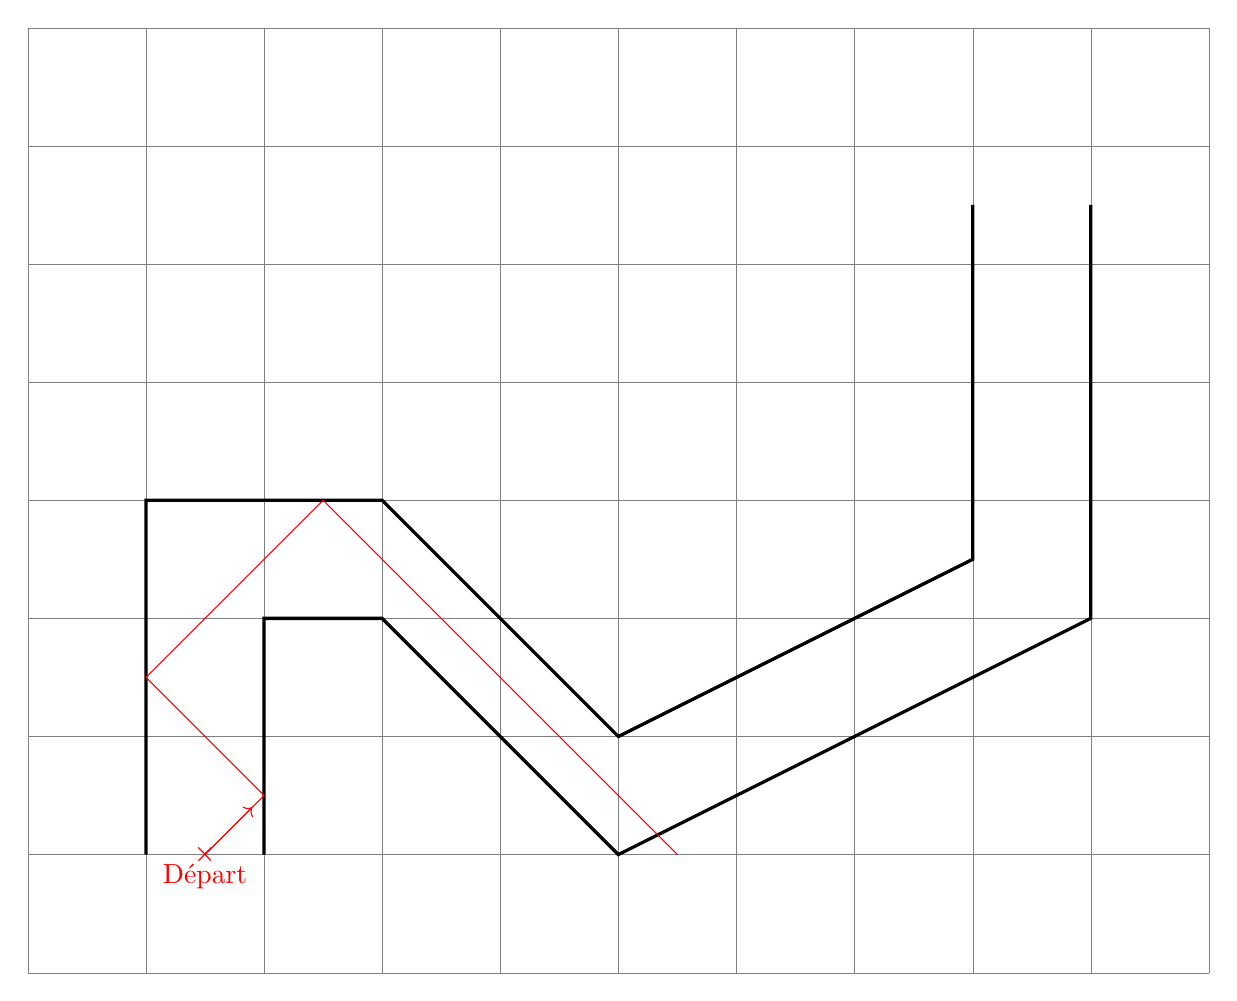
\begin{tikzpicture}[scale=1.5]
		\draw[ultra thin,gray] (0,0) grid (10,8);

		\draw[very thick] (1,1)
		-- ++(0,3)
		-- ++(2,0)
		-- ++(2,-2)
		-- ++(3,1.5)
		-- ++(0,3);

		\draw[very thick] (2,1)
		-- ++(0,2)
		-- ++(1,0)
		-- ++(2,-2)
		-- ++(4,2)
		-- ++(0,3.5);

		\coordinate (Start) at (1.5,1);

		\node[red] at (Start) {×};
		\node[red,below] at (Start) {Départ};
		\draw[red,->] (Start) -- ++(0.4,0.4);

		\draw[red] (Start)
		-- ++(0.5,0.5)
		-- ++(-1,1)
		-- ++(1.5,1.5)
		-- ++(3,-3);
	\end{tikzpicture}
\end{center}

\end{document}